%From https://egu2018.eu/PICO_how-to_guide_to_PICO.pdf
%Abstracted and templated by Brian Ballsun-Stanton, Macquarie University.
%original template by https://github.com/snowtechblog/pico-latex-presentation by Anselm Köhler

\documentclass[unknownkeysallowed,usepdftitle=false, aspectratio=169, parskip=full]{beamer}
% unknownkeysallowed is needed for mac and the newer latex version -> is more picky than before...
\usetheme[headheight=1cm,footheight=2cm]{boxes}
%\usetheme{default}


\usepackage{default}
\usepackage{graphicx}
%example pictures created via: http://lorempixel.com/1200/800/cats/Figure2/. Credit to http://lorempixel.com/images.php

%\usepackage[colorlinks=true,linkcolor=blue]{hyperref}

\usepackage{hyperref}
\hypersetup{
    colorlinks=true,
    linkcolor=blue,
    filecolor=magenta,      
    urlcolor=cyan,
}

\usepackage{epsfig}
\usepackage{siunitx}
\usepackage{color}
\usepackage{ifthen}
%usepackage{ragged2e}

\usepackage[T1]{fontenc}
\usepackage[utf8]{inputenc}
%https://tex.stackexchange.com/a/203804/5483

\usepackage[activate={true,nocompatibility},final,tracking=true,kerning=true,spacing=true,factor=1100,stretch=10,shrink=10]{microtype} % http://www.khirevich.com/latex/microtype/
\microtypecontext{spacing=nonfrench}

\usepackage{lipsum} % for dummy text only
\usepackage[UKenglish]{babel} %https://tex.stackexchange.com/a/27743 
\usepackage[pangram]{blindtext} % https://tex.stackexchange.com/a/48411

%\usepackage{parskip} % from https://tex.stackexchange.com/q/11622
%\setlength{\parskip}{12pt} 

%\setparsizes{\parindent}{12pt}{\parfillskip}

%\usepackage{etoolbox} % as per https://tex.stackexchange.com/a/24331
%\appto\chapterheadendvskip{\vspace{-1\parskip}}
%\setparsizes{\parindent}{50pt plus 20pt minus 30pt}{\parfillskip}

\setbeamertemplate{navigation symbols}{}%remove navigation symbols
\setbeamersize{text margin left=1cm,text margin right=1cm}

% some colors
\definecolor{grau}{gray}{.5}
\definecolor{slfcolor}{rgb}{0,0.6274,0.8353}
\definecolor{wslcolor}{rgb}{0,0.4,0.4}

% setup links
\hypersetup{%
	%linkbordercolor=green,%
	colorlinks=false,%
	pdfborderstyle={/S/U/W 0},%
	%pdfpagemode=FullScreen,%
	pdfstartpage=4%
	}

% setup some fonts
\setbeamerfont{title}{series=\bfseries, size=\small}
\setbeamerfont{author}{size*={5pt}{0pt}}
\setbeamerfont{institute}{size*={3pt}{0pt}}
\setbeamerfont{bodytext}{size=\scriptsize}
	
% Title setup	
\title{Robust feedback tracking for Docx et al}
\author{Jeremy Amin\inst{1} (\texttt{jeremy.amin@stuents.mq.edu.au})}

% add title in headbox
\setbeamertemplate{headline}
{\leavevmode
\begin{beamercolorbox}[width=1\paperwidth]{head title}
  % LOGO
  \vspace{.1cm}
  \begin{columns}[t, totalwidth=\textwidth]
  \begin{column}[c]{1.5cm}
     
\includegraphics[width=1cm]{Logos/pandoc-image.png}
  \end{column}
  % TITLE
   \begin{column}[c]{10.6cm}
   
   \centering \usebeamerfont{title} \textcolor{slfcolor}{\inserttitle} \\
   \centering \usebeamerfont{author} \color[rgb]{0,0,0} \insertauthor \\
   \vspace{-0.05cm}
   \centering \usebeamerfont{institute} \insertinstitute
  \end{column}
  % PICTURE
  \begin{column}[c]{1cm}
    \hspace{0.005cm}
    
\includegraphics[width=1cm]{Logos/git-image.png}
  \end{column}
  \end{columns}
  {\color{slfcolor}\hrule height 1pt\vspace{0.1cm}}
\end{beamercolorbox}%
}

% setup the navigation in footbox
% first set some button colors
\newcommand{\buttonactive}{\setbeamercolor{button}{bg=wslcolor,fg=white}}
\newcommand{\buttonpassive}{\setbeamercolor{button}{bg=slfcolor,fg=black}}
% now set up that the one active one gets the new color.
\newcommand{\secvariable}{nothing}
% therefore we write before each section (well, everything which should be part of the navi bar)
% the variable \secvariable to any name which is in the next function ...
\newcommand{\mysection}[1]{\renewcommand{\secvariable}{#1}
}
% ... compaired to strings in the following navibar definition ...
\newcommand{\tocbuttoncolor}[1]{%
 \ifthenelse{\equal{\secvariable}{#1}}{%
    \buttonactive}{%
    \buttonpassive}
 }
% ... here we start to set up the navibar. each entry is calling first the function \tocbuttoncolor with the argument which should be tested for beeing active. if active, then change color. afterwards the button is draw. so to change that, you need to change the argument in \toc..color, the first in \hyperlink and before each frames definition... A bit messed up, but works...
\newlength{\buttonspacingfootline}
\setlength{\buttonspacingfootline}{-0.2cm}
\setbeamertemplate{footline}
{\leavevmode
\begin{beamercolorbox}[width=1\paperwidth]{head title}
  {\color{slfcolor}\hrule height 1pt}
  \vspace{0.05cm}
  % set up the buttons in an mbox
  \centering \mbox{
    \tocbuttoncolor{abstract}
    \hyperlink{abstract}{\beamerbutton{2 Minute Madness}}
    \tocbuttoncolor{radar}
    \hspace{\buttonspacingfootline}
      \hyperlink{radar}{\beamerbutton{Section 1}}

    \tocbuttoncolor{line}
    \hspace{\buttonspacingfootline}
      \hyperlink{line}{\beamerbutton{Section 2}}
    \tocbuttoncolor{major}
    \hspace{\buttonspacingfootline}
      \hyperlink{major}{\beamerbutton{Section 3}}
    \tocbuttoncolor{slab}
    \hspace{\buttonspacingfootline}
      \hyperlink{slab}{\beamerbutton{Section 4}}
    \tocbuttoncolor{minor}
    \hspace{\buttonspacingfootline}
      \hyperlink{minor}{\beamerbutton{Section 5}}
    \tocbuttoncolor{conclusion}
    \hspace{\buttonspacingfootline}
      \hyperlink{conclusion}{\beamerbutton{Conclusion}}
    % this last one should normaly not be used... it will open the preferences to change the 
    % behaviour of the acrobat reader in fullscreen -> usefull in pico...
    \setbeamercolor{button}{bg=white,fg=black}
    % for presentation
    %\hspace{-0.1cm}\Acrobatmenu{FullScreenPrefs}{\beamerbutton{\#}}
    % for upload
    
     
%\Acrobatmenu{FullScreenPrefs}{\vspace{0.3cm}\hspace{0.24cm}\mbox{%
%      \includegraphics[height=0.04\textheight,keepaspectratio]{%
%	  figure/CreativeCommons_Attribution_License.eps}%
%	  }}
   }
    \vspace{0.05cm}
\end{beamercolorbox}%
}


\begin{document}


%%%%%%%%%%%%%%%%%%%%%%%%%%%%%%%%%%%%%%%%%%%%%%%%%%%%%%%%%%%%%%%%%%%%%%%%%%
\mysection{abstract}
%%%%%%%%%%%%%%%%%%%%%%%%%%%%%%%%%%%%%%%%%%%%%%%%%%%%%%%%%%%%%%%%%%%%%%%%%%
\begin{frame}\label{\secvariable}

\usebeamerfont{bodytext}


\parbox{\linewidth}{

\boldsymbol{PROBLEM:} We cannot control how our peers prefer to receive and provide feedback on our work. Docx, TeX, txt, PDF, ODT, pen and paper...


\vspace{12pt}

\boldsymbol{WHY?:} Many different types of file in many locations with little to no cohesion

 \vspace{12pt}
 
\boldsymbol{SOLUTION:} A workflow for tracking feedback from multiple different file types in an easy to do way which allows for:
\begin{itemize}
    \item Quick conversions from one file type to another and vice versa
    \item Creating and maintaining a history of all feedback. Dated with time. Ability to access any version of the document and/or comments received.

\end{itemize}

 \vspace{12pt}
 
\boldsymbol{}
}


   
\end{frame}

\begin{frame}\label{\secvariable}
  \begin{columns}[t]
  %https://tex.stackexchange.com/a/7452/5483
  \begin{column}[c]{0.45\textwidth}
%http://lorempixel.com/1200/800/cats/Figure2/     
%http://lorempixel.com/1200/800/cats/Figure3/
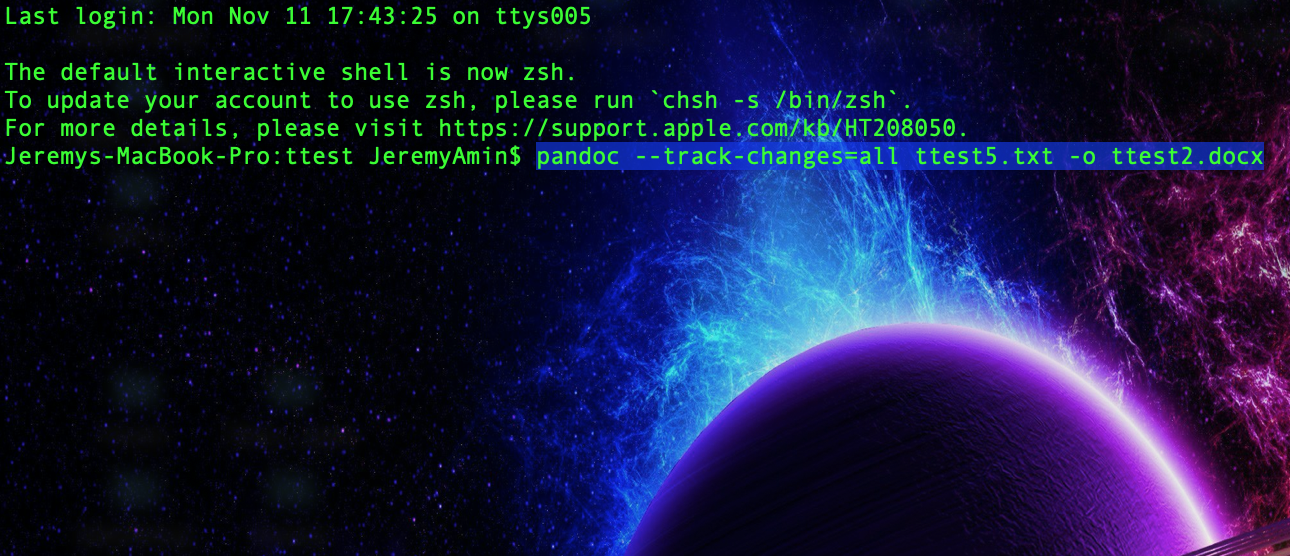
\includegraphics[width=1\textwidth,height=0.5\textheight,keepaspectratio]{%
Screenshots/Shell-pandoc-command.png}\\
\vspace{12pt}
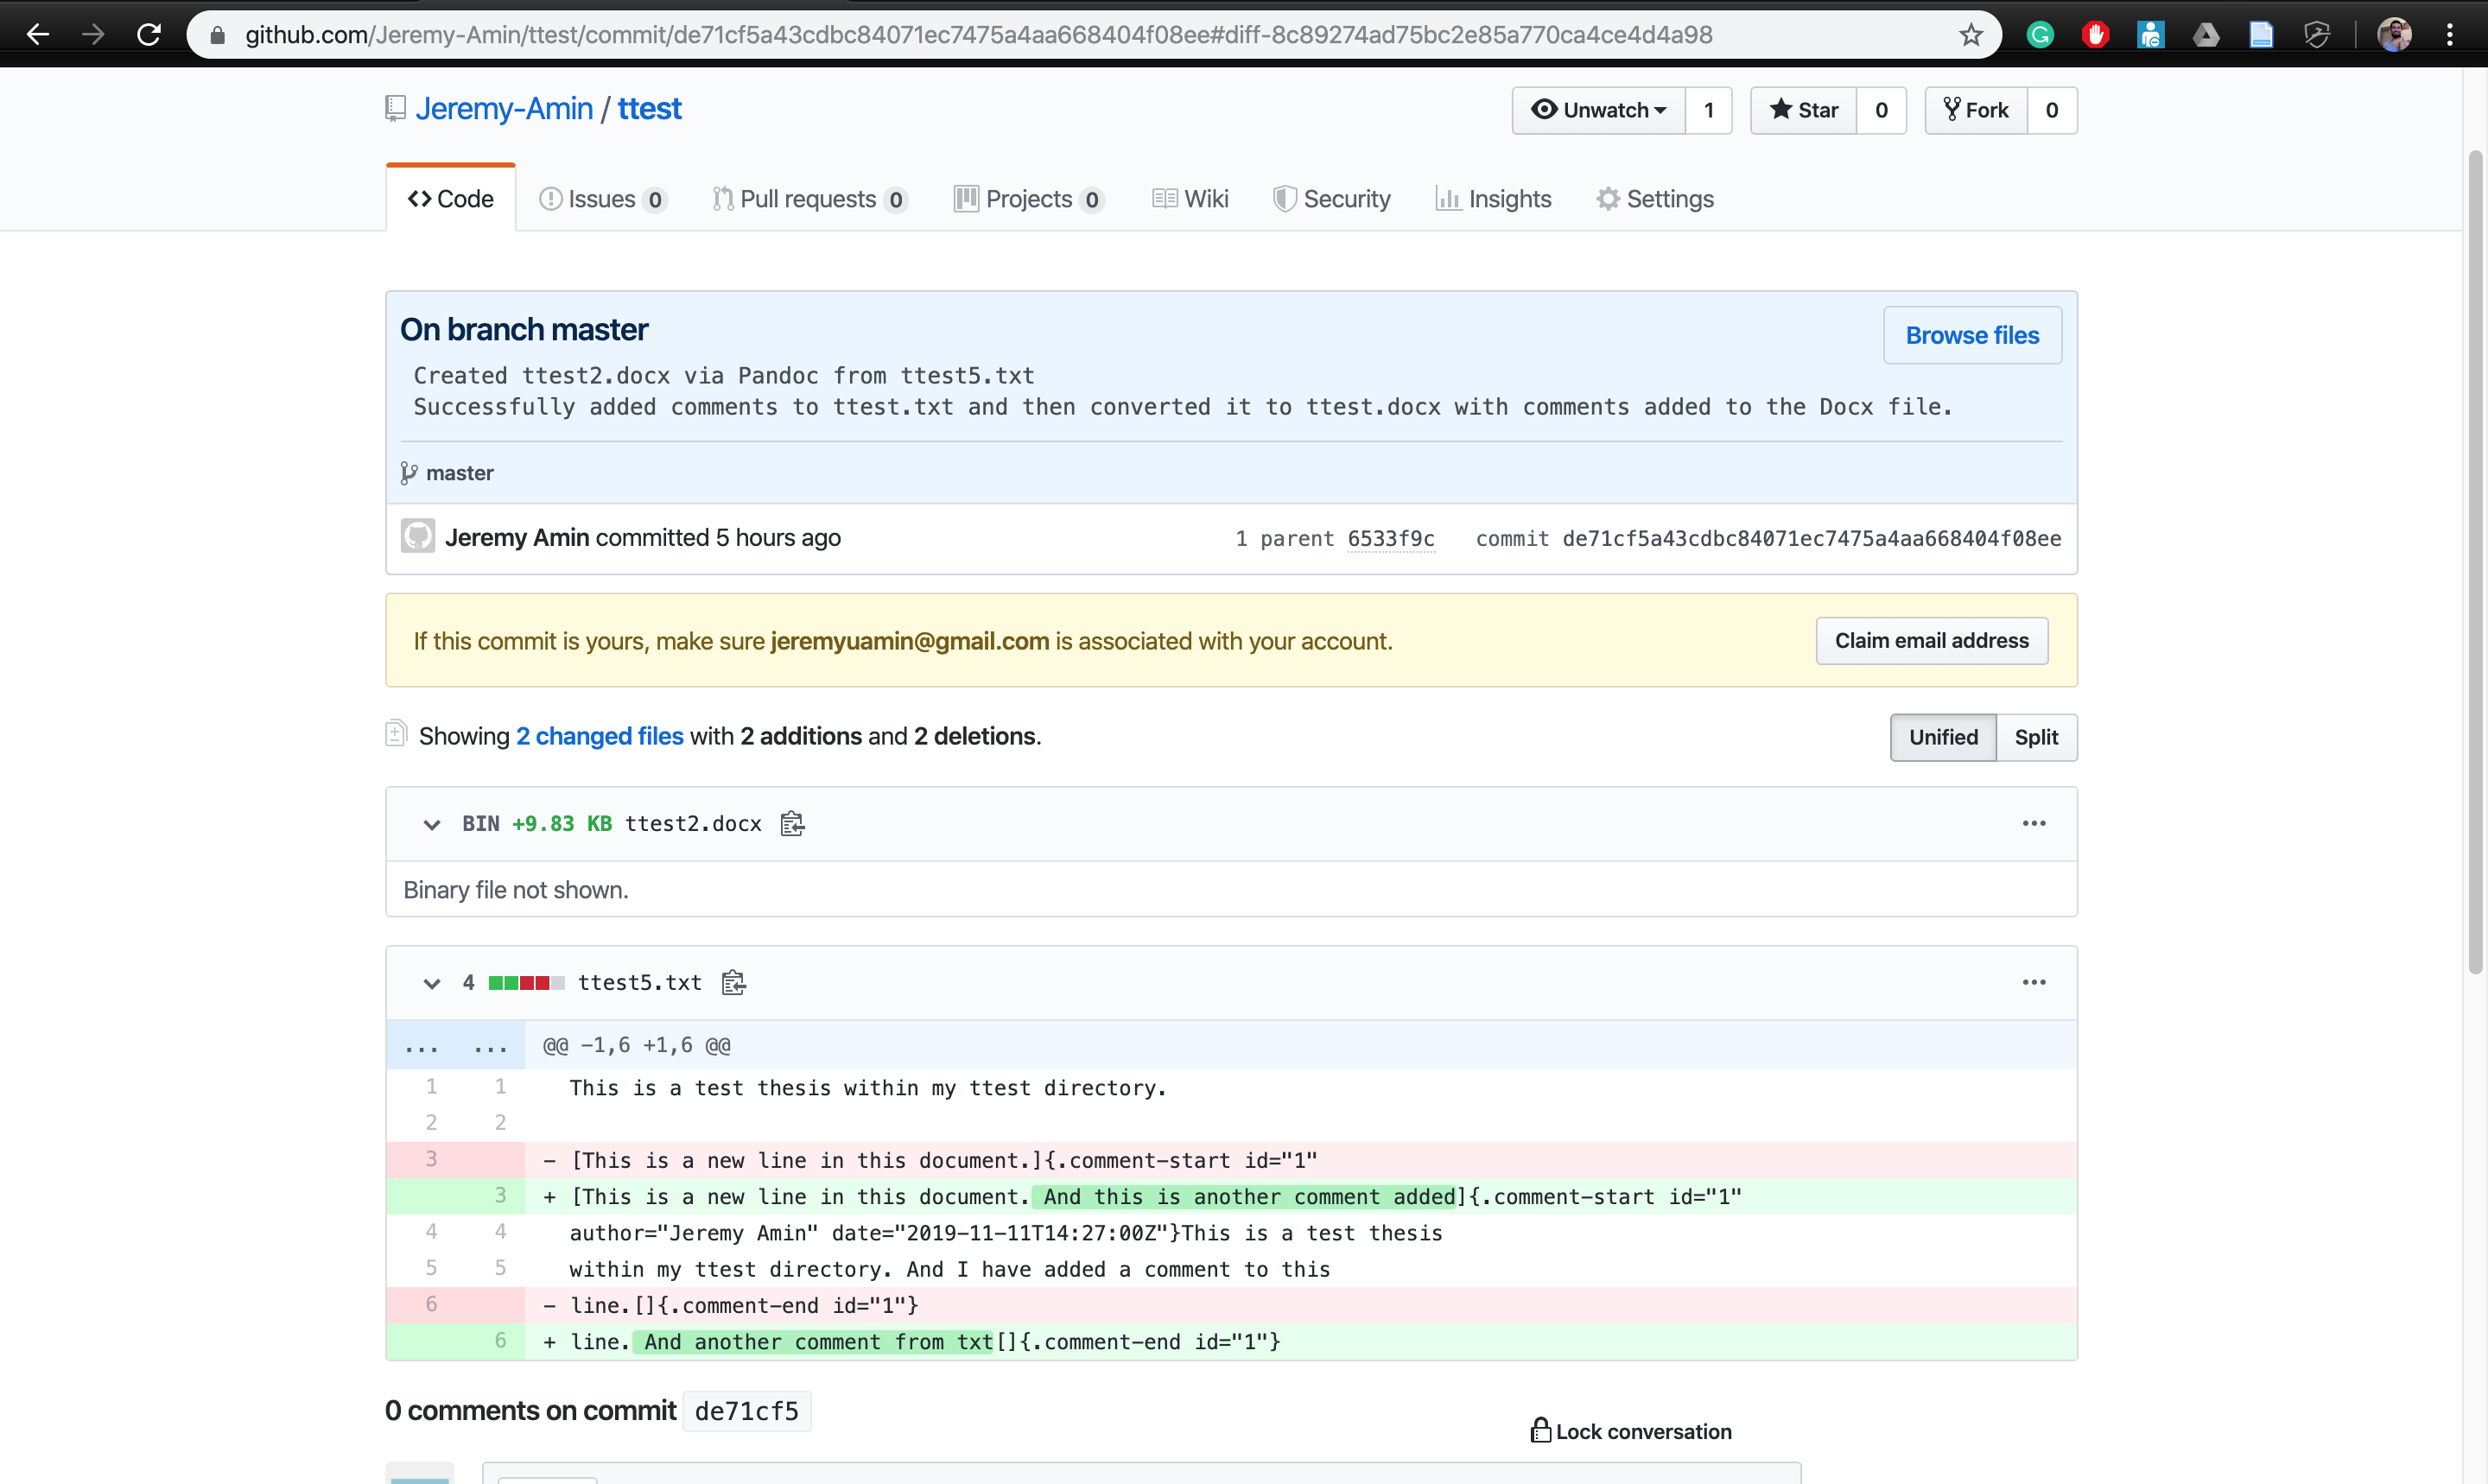
\includegraphics[width=1\textwidth,height=0.5\textheight,keepaspectratio]{%
Screenshots/GHttest5txtcommit2.png}
    \end{column}
    \begin{column}[c]{0.45\textwidth}
    \parbox{\linewidth}{
    \begin{itemize}
        \item Terminal - Shell
        \item Pandoc
        \item Git
        \item GitHub 
    \end{itemize}
      
      
      \vspace{12pt}
      }
    \end{column}
    
  \end{columns}

  
\end{frame}

%%%%%%%%%%%%%%%%%%%%%%%%%%%%%%%%%%%%%%%%%%%%%%%%%%%%%%%%%%%%%%%%%%%%%%%%%%
\mysection{radar}
%%%%%%%%%%%%%%%%%%%%%%%%%%%%%%%%%%%%%%%%%%%%%%%%%%%%%%%%%%%%%%%%%%%%%%%%%%
\begin{frame}\label{\secvariable}
\begin{center}
  \vspace{-0.5cm}
  %http://lorempixel.com/1200/800/cats/Figure4/
 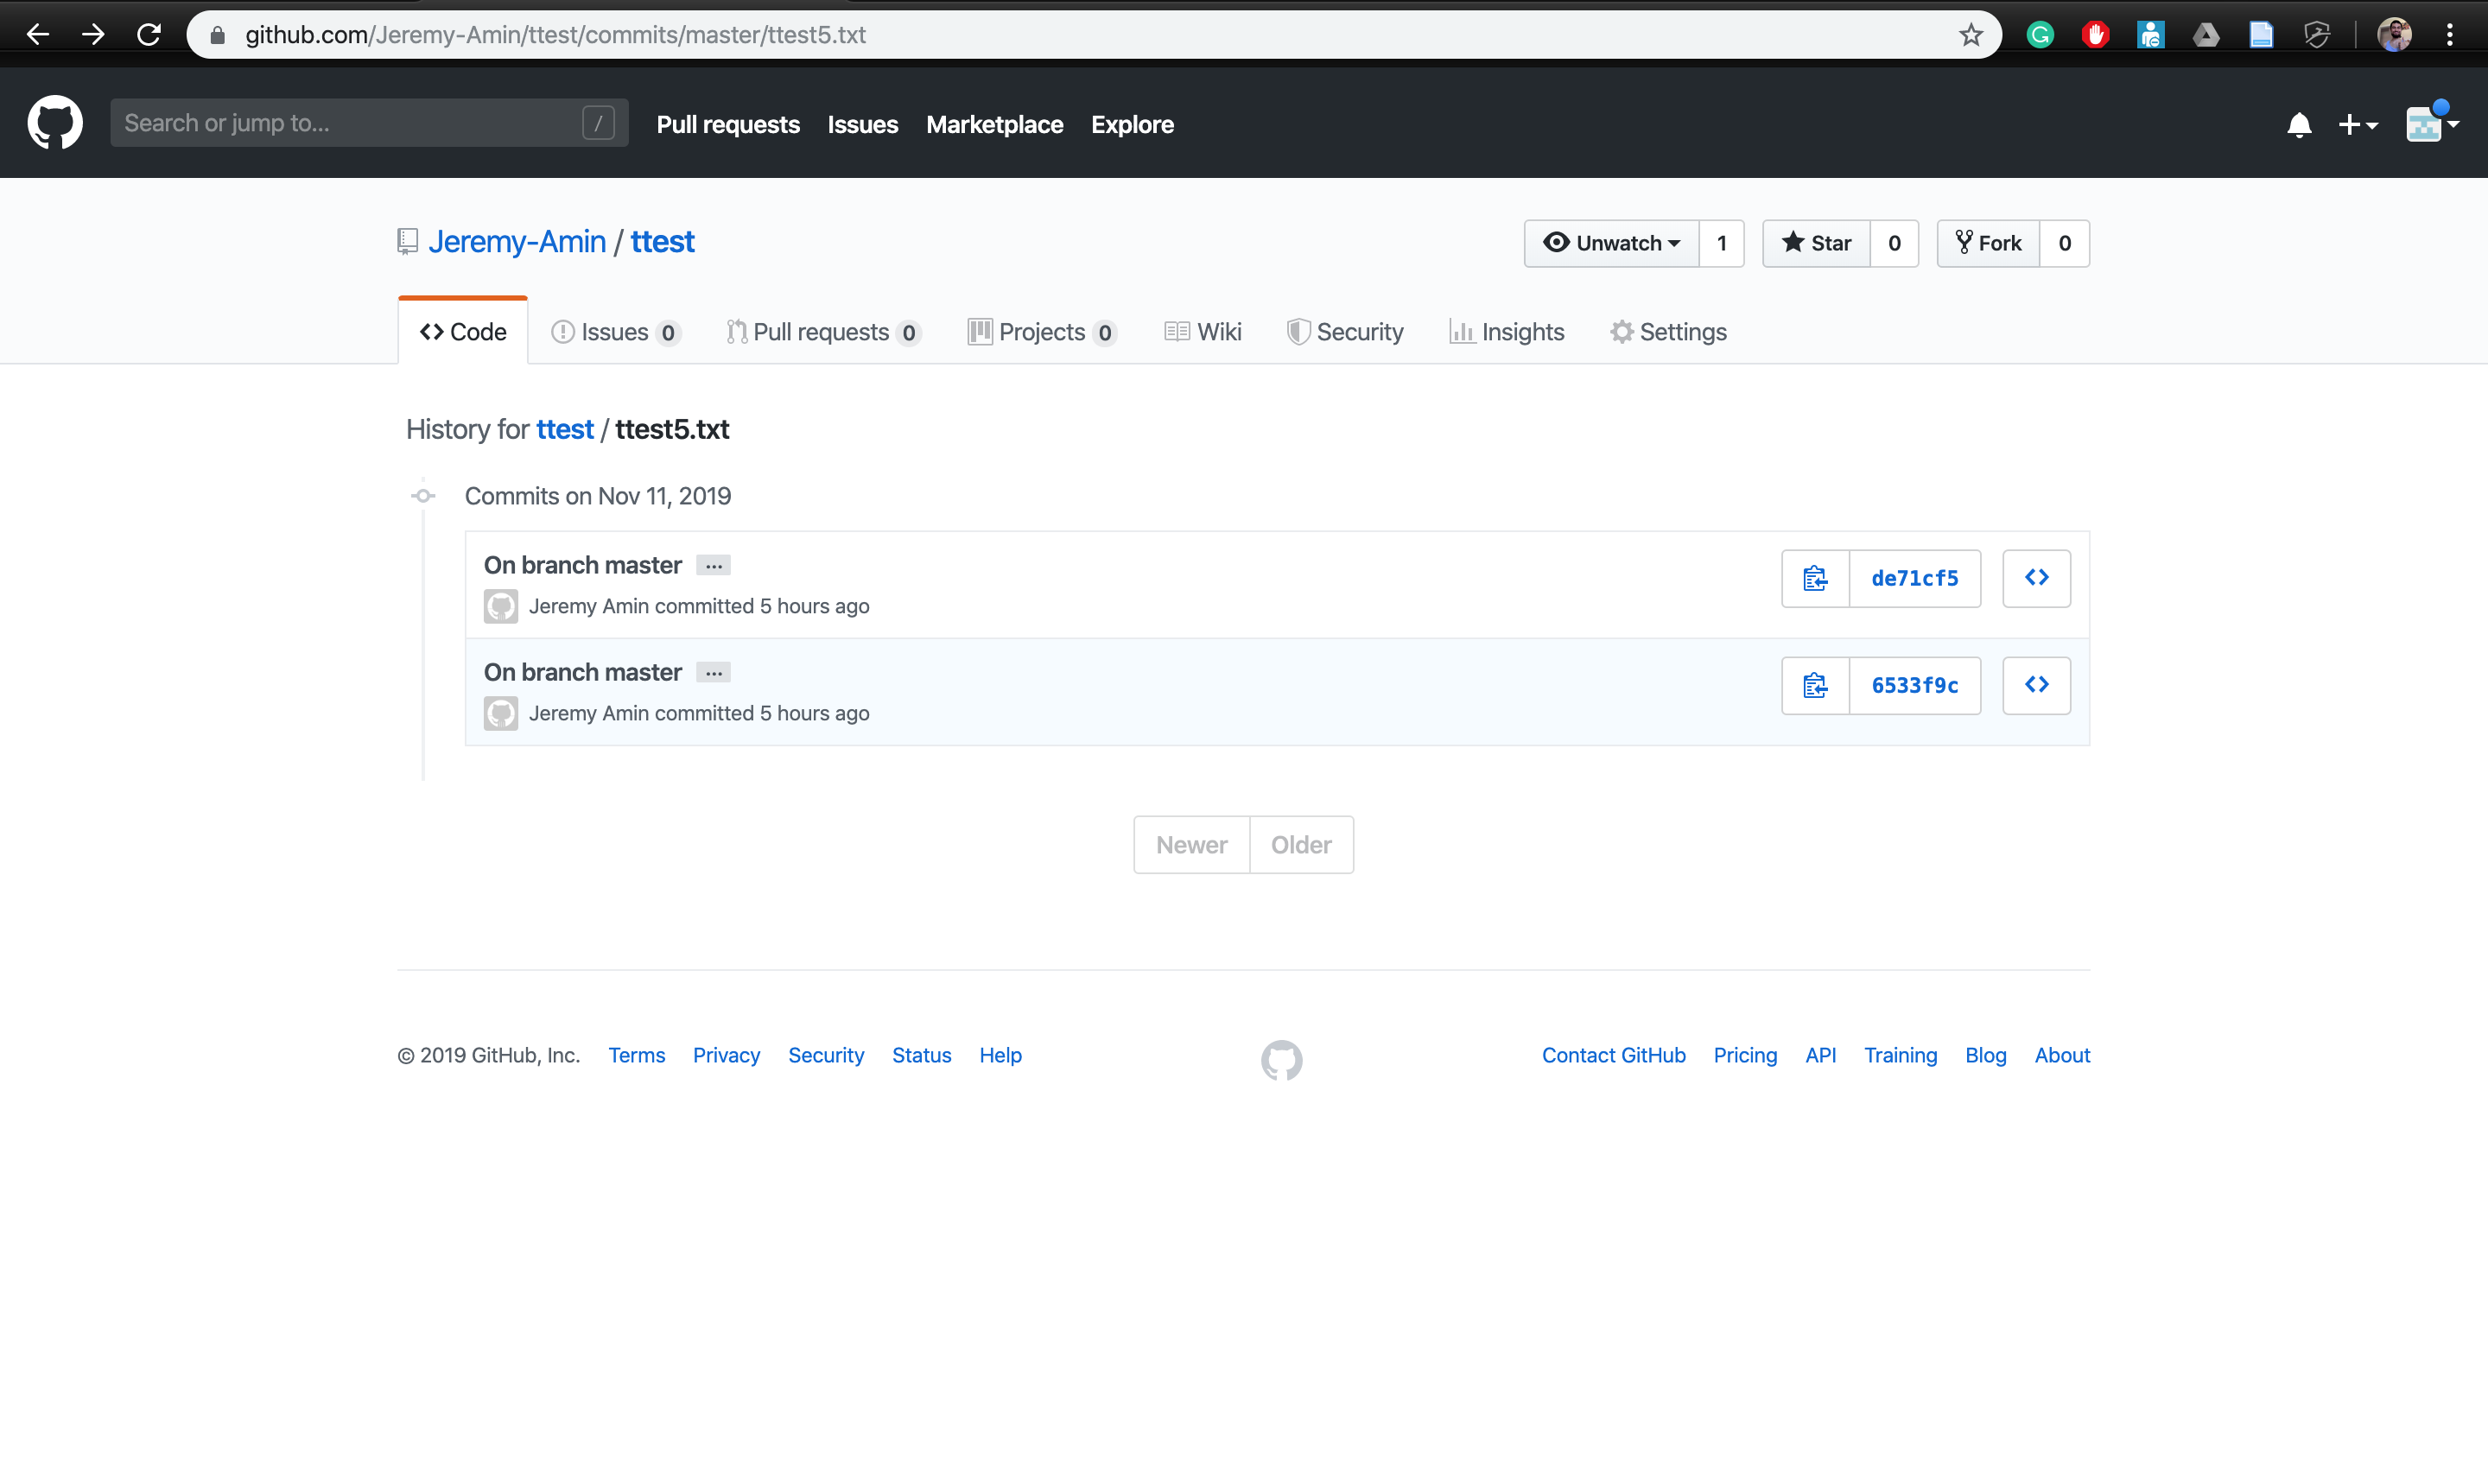
\includegraphics[width=1\textwidth,height=0.75\textheight,keepaspectratio]{%
  Screenshots/GHttest5txthist.png}
\end{center}
  \vspace{-0.5cm}
  
  Pandoc preserves the edits for the new Docx file!

%Screenshots/GHttest5txthist.png
\end{frame}

%%%%%%%%%%%%%%%%%%%%%%%%%%%%%%%%%%%%%%%%%%%%%%%%%%%%%%%%%%%%%%%%%%%%%%%%%%
\mysection{line}
%%%%%%%%%%%%%%%%%%%%%%%%%%%%%%%%%%%%%%%%%%%%%%%%%%%%%%%%%%%%%%%%%%%%%%%%%%
\begin{frame}\label{\secvariable}
\begin{center}
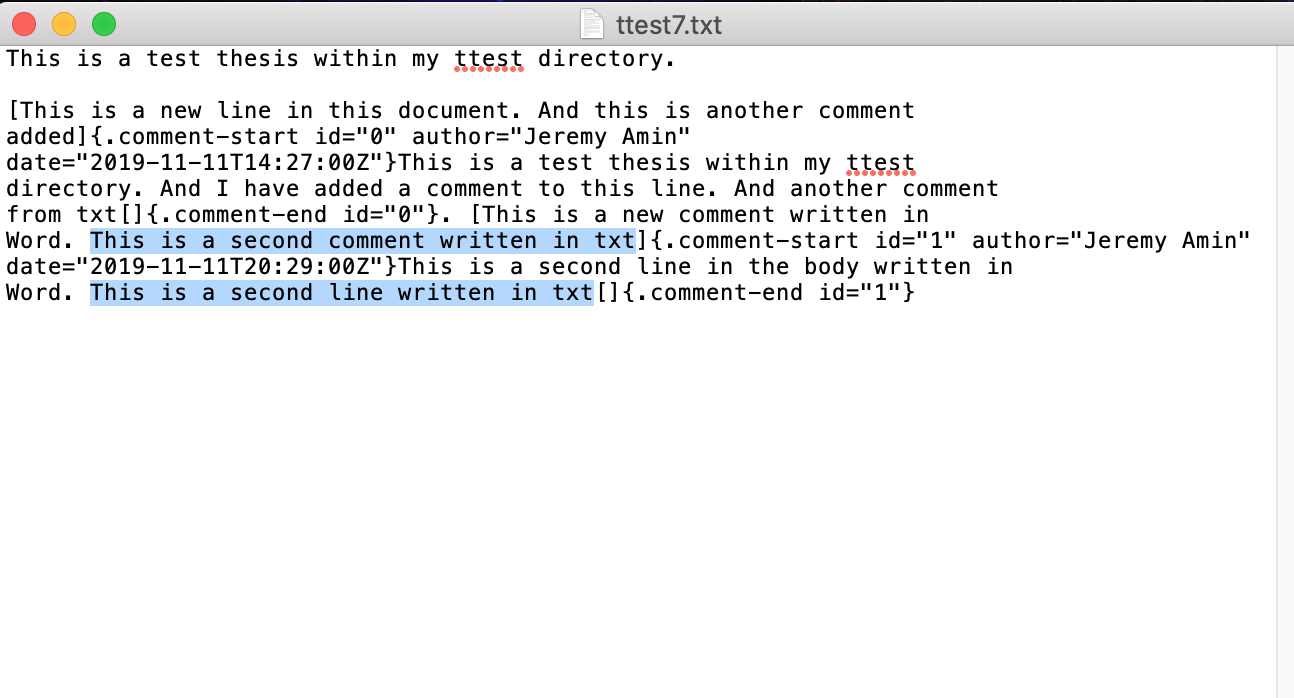
\includegraphics[width=1\textwidth,height=0.75\textheight,keepaspectratio]{%
Screenshots/txt-word-edit.png}
\end{center}
    \parbox{\linewidth}{

A txt file converted from a Docx via Pandoc in Shell. Highlighted sections are written in txt, and when run through Pandoc from .txt to .docx...
}
\end{frame}

%%%%%%%%%%%%%%%%%%%%%%%%%%%%%%%%%%%%%%%%%%%%%%%%%%%%%%%%%%%%%%%%%%%%%%%%%%
\mysection{major}
%%%%%%%%%%%%%%%%%%%%%%%%%%%%%%%%%%%%%%%%%%%%%%%%%%%%%%%%%%%%%%%%%%%%%%%%%%
\begin{frame}\label{\secvariable} %%Eine Folie
\begin{center}
  \vspace{-0.5cm}
  %http://lorempixel.com/1200/800/cats/Figure4/
 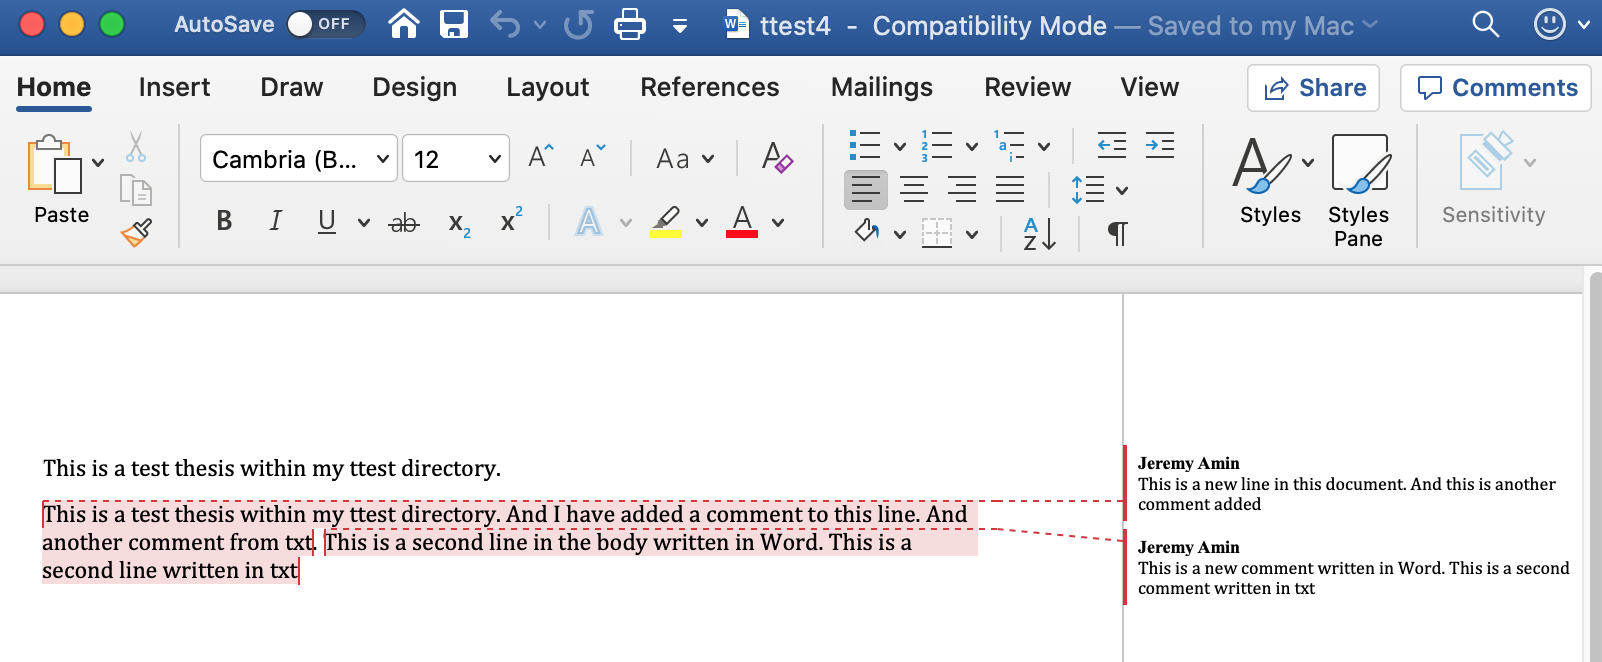
\includegraphics[width=1\textwidth,height=0.75\textheight,keepaspectratio]{%
  Screenshots/Word-doc-with-txt-comment-edit.png}
\end{center}
  \vspace{-0.5cm}
  
  I edited in the last line in the body and the second comment from a txt file. Pandoc converted it to this Docx with the changes transferred successfully.

\end{frame}

%%%%%%%%%%%%%%%%%%%%%%%%%%%%%%%%%%%%%%%%%%%%%%%%%%%%%%%%%%%%%%%%%%%%%%%%%%
\mysection{slab}
%%%%%%%%%%%%%%%%%%%%%%%%%%%%%%%%%%%%%%%%%%%%%%%%%%%%%%%%%%%%%%%%%%%%%%%%%%
\begin{frame}\label{\secvariable}
%http://lorempixel.com/1200/800/cats/Figure6/

\begin{center}
  \vspace{-0.5cm}
  %http://lorempixel.com/1200/800/cats/Figure4/
 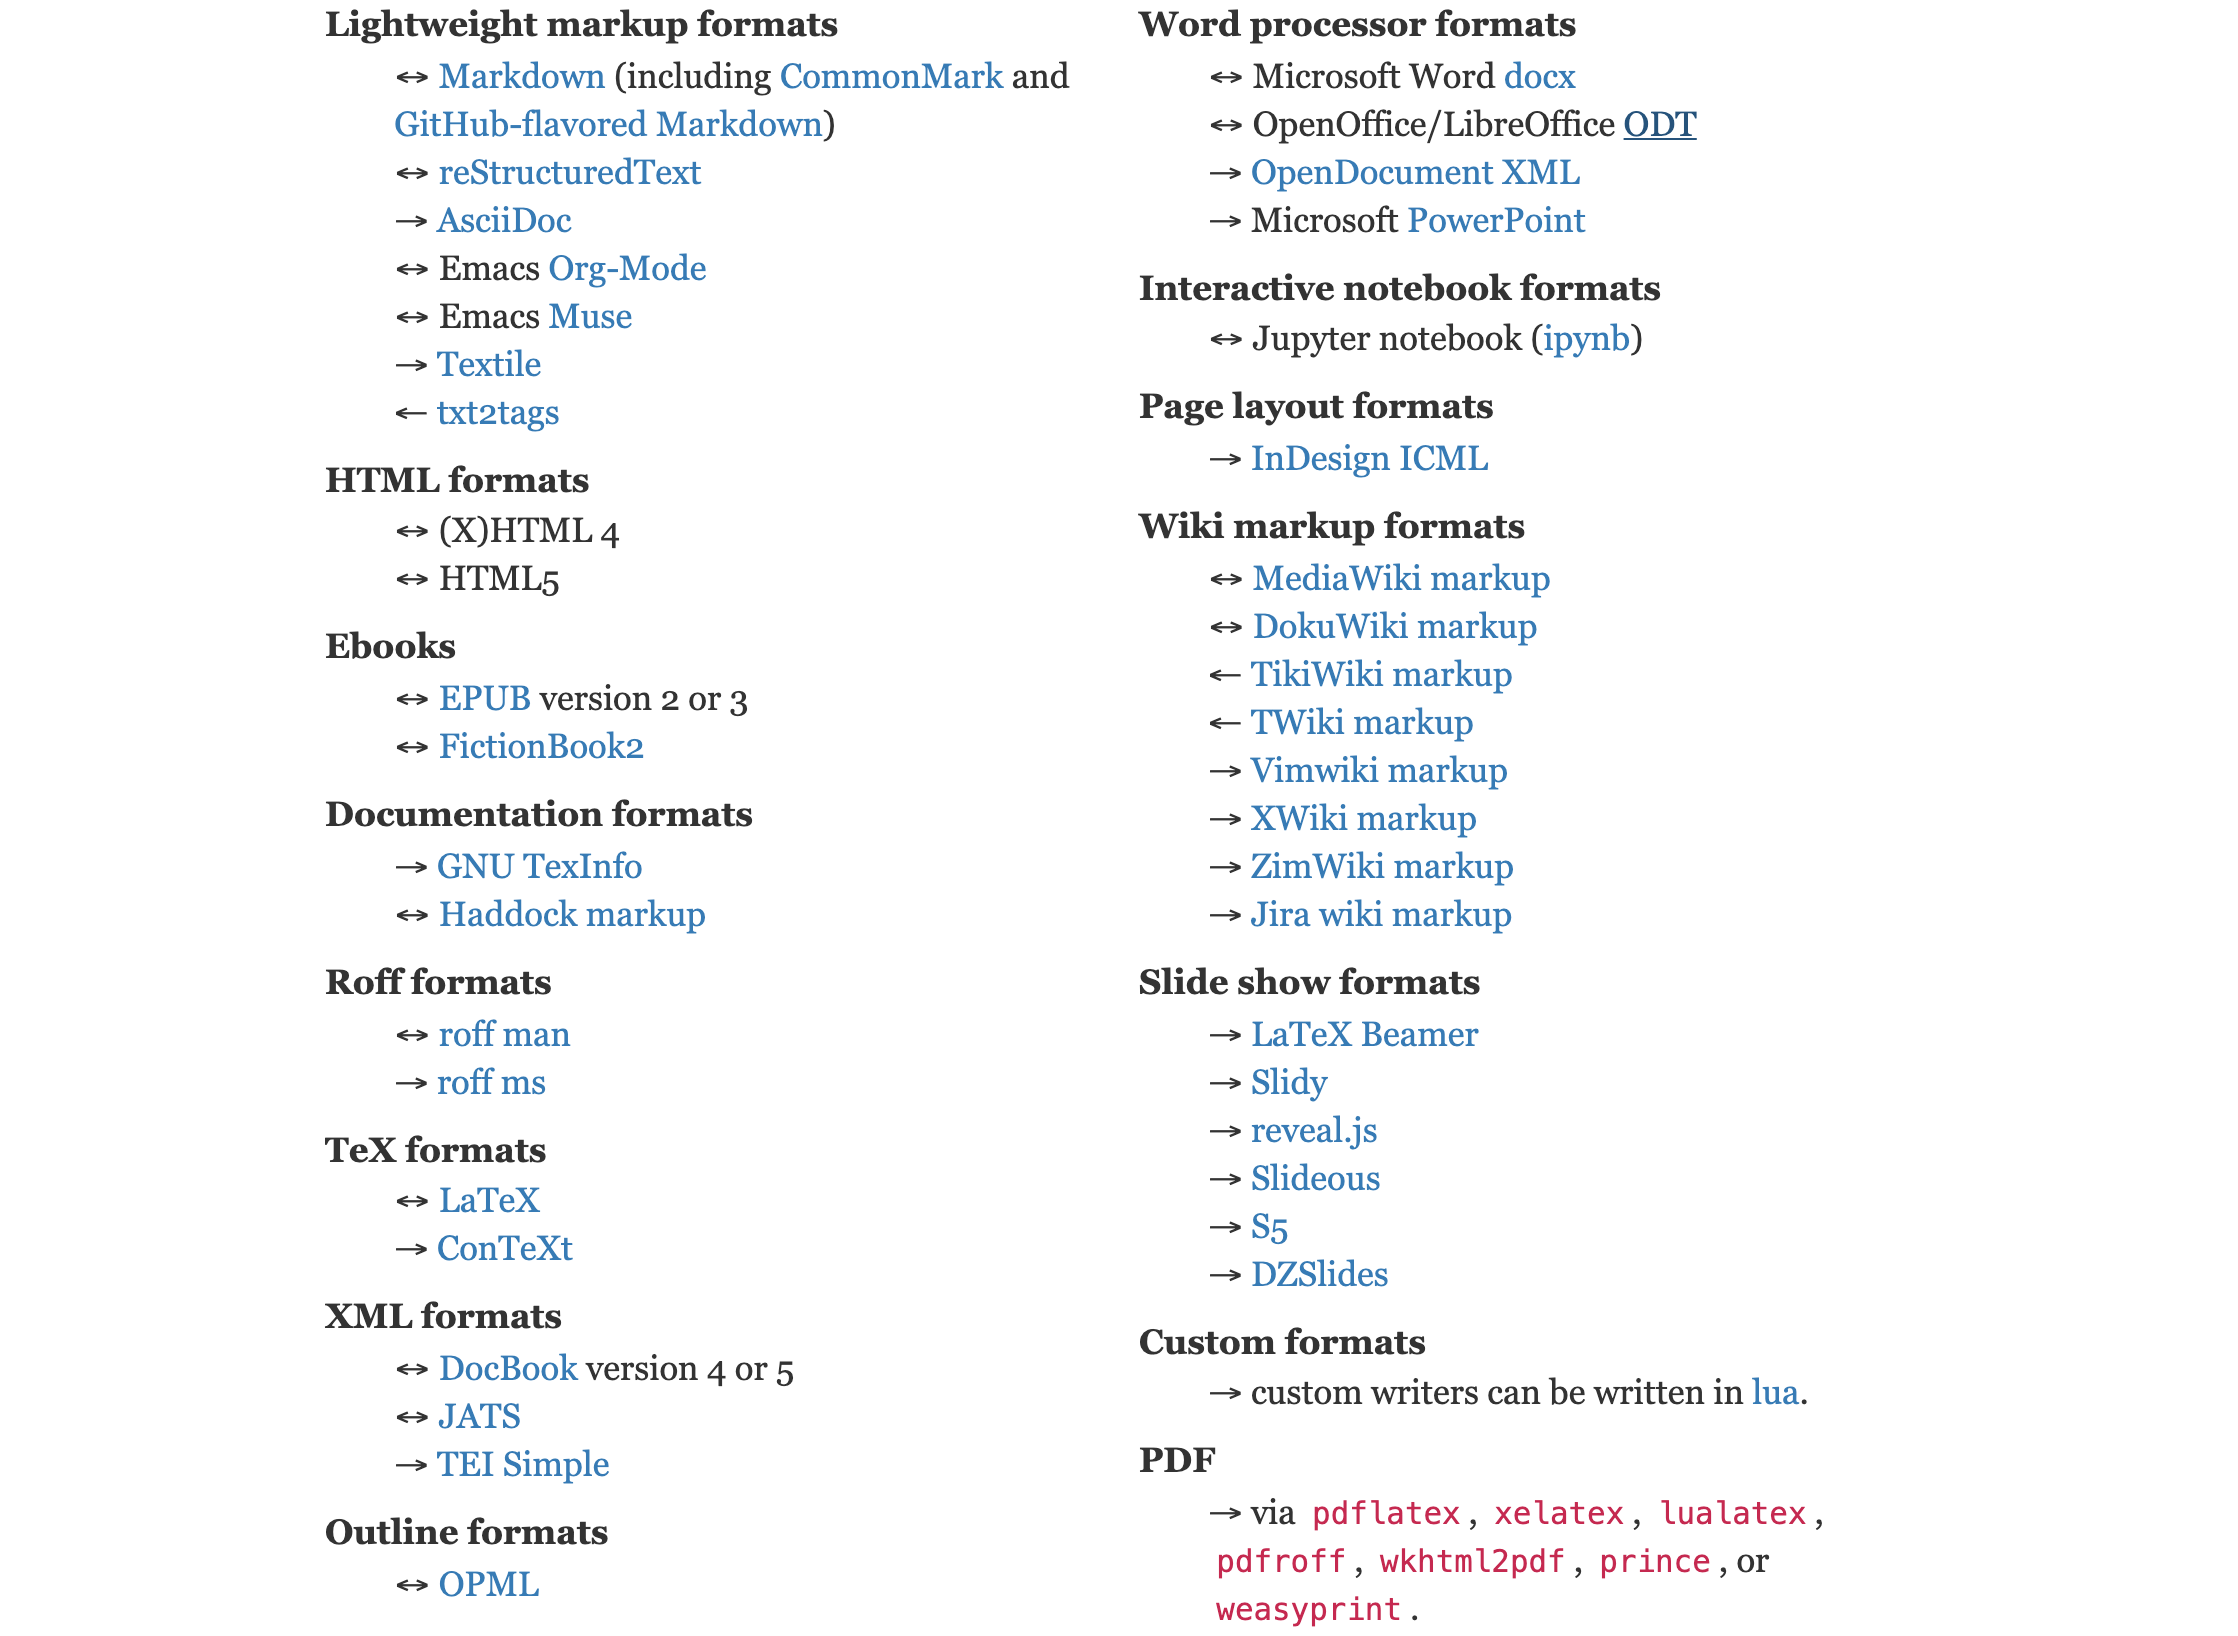
\includegraphics[width=1\textwidth,height=0.75\textheight,keepaspectratio]{%
  Screenshots/pandoc-convlist.png}
\end{center}
  \vspace{-0.5cm}
  
  List of conversions \href{https://pandoc.org/index.html}{Pandoc} can do 

\end{frame}



\begin{frame}\label{slabtable}
\begin{columns}
\begin{column}[t]{1.1\textwidth}
\hyperlink{slab}{\beamerbutton{\dots back to figure}}\\
Morbi mauris turpis, ornare eu elit quis, pulvinar bibendum sapien. Nulla vel justo id dui aliquam blandit. Etiam pellentesque ac nisl ut suscipit. 


%Table from original template.

\vspace{0.3cm}
\end{column}
\end{columns}
\usebeamerfont{bodytext}
 
\vspace{0.2cm}

\end{frame}




%%%%%%%%%%%%%%%%%%%%%%%%%%%%%%%%%%%%%%%%%%%%%%%%%%%%%%%%%%%%%%%%%%%%%%%%%%
\mysection{minor}
%%%%%%%%%%%%%%%%%%%%%%%%%%%%%%%%%%%%%%%%%%%%%%%%%%%%%%%%%%%%%%%%%%%%%%%%%%
\begin{frame}\label{\secvariable} %%Eine Folie
\begin{center}
%http://lorempixel.com/1200/800/cats/Figure7/
\includegraphics[width=1\textwidth,height=0.7\textheight,keepaspectratio]{%
figure/figure7.png}
\end{center}
\vspace{-0.2cm}

\end{frame}

%%%%%%%%%%%%%%%%%%%%%%%%%%%%%%%%%%%%%%%%%%%%%%%%%%%%%%%%%%%%%%%%%%%%%%%%%%

%%%%%%%%%%%%%%%%%%%%%%%%%%%%%%%%%%%%%%%%%%%%%%%%%%%%%%%%%%%%%%%%%%%%%%%%%%
\begin{frame}\label{\secvariable}

%
Websites
    \begin{itemize}
        \item \href{https://pandoc.org/index.html}{Pandoc}
        \item \href{https://github.com/}{GitHub}
        \item \href{https://git-scm.com/}{Git}
    \end{itemize}

\end{frame}

%%%%%%%%%%%%%%%%%%%%%%%%%%%%%%%%%%%%%%%%%%%%%%%%%%%%%%%%%%%%%%%%%%%%%%%%%%
\mysection{conclusion}
%%%%%%%%%%%%%%%%%%%%%%%%%%%%%%%%%%%%%%%%%%%%%%%%%%%%%%%%%%%%%%%%%%%%%%%%%%
\begin{frame}\label{\secvariable}
  
\end{frame}



\end{document}
